%
% Chapter "Transaction Management"
%
% Description of cluster-wide MVCC and transaction management in \XC.
%


%========= SECTION SECTION ===================================================

\section{\label{sec:cw-mvcc}Cluster-wide MVCC}

  \XC's transaction management is compliant with ACID and ensures atomic visibility for
  multi-node read transactions among the cluster.
  This feature is achieved by implementing cluster-wide MVCC.
  \XC{} basically uses \PG's MVCC mechanism implemented in \file{src/backend/utils/time/tqual.c}:
  visibility is checked by \texttt{xmin}, \texttt{xmax}, \textbf{CLOG} and transaction snapshot
  (sometimes cmin and cmax are included.)
  \XC{} just extends \PG's mechanism to assign the transaction ID and to feed snapshot to global.
  The external component which feeds global transaction information is called Global Transaction
  Manager (GTM), which clusetr-wide MVCC depends upon.
  It was implemented separately from the core of coordinator and datanode.
  The source code will be found in
  \file{src/gtm/main} as described at section~\ref{sec:gtm}, page~\pageref{sec:gtm}.
  
  When a user issues a DML statement to a coordinator, the coordinator obtains a global transaction
  ID (GXID) and a global transaction snapshot from GTM and send it to datanodes.
  Datanodes manipulate their database using GXID and snapshot from the coordinator.
  In such manner, datanodes share the same transaction context and a transaction
  can maintain atomic and uniform visibility
  when it runs in more than one coordinators and datanodes.
  At the end of transaction, if more than one nodes are involved in the updates, the coordinator commits
  the transaction using 2PC protocol implicitly.
  By keeping track with global transaction status, coordinator reports global transaction status to GTM.
  
  Visibility check sometimes uses transaction-local command ID generated by coordinators.
  It is also sent to datanodes before each command is shipped.
  If the command ID is advanced locally in some of involved datanodes,
  they notify the change to the coordinator. 
  
  The detailed modifications to the transaction mechanism is described in section~\ref{sec:gtx}, page~\pageref{sec:gtx}.
  
  \XC{} supports all transaction isolation levels implemented in \PG.
  If the transaction isolation level is \texttt{REPEATABLE READ}, one snapshot will be obtained and used
  throughout the transaction.
  If the isolation mode is \texttt{READ COMMITTED}, the coordinator obtains fresh snapshot for each statement.
  Please note that this snapshot is used for more than one statements if one statment is devided into
  multiple ones by the planner.
  \footnote{
	  I thought \XC{} doesn't support \texttt{REPEATABLE READ}. Doesn't it? -- Saito --\\
	  -- Koichi --\\
	  As design, it does.
	  Sometime after 1.0 was released, new bug was introduced to disable \texttt{REPEATABLE READ}.
	  It is not a design issue but a bug.
	  In terms of \texttt{SERIALIZABLE}, predicate lock will work corretly with distributed tables.
	  In the case of replicated tables, I believe each read in different datanode will leave their
	  predicate lock.
	  Conflicting writes will be detected in some of the datanodes which ends up with transaction
	  failure.
	  If it is true, \XC{} can support \texttt{SERIALIZABLE} isolation level too.
  }.
  
  Some small changes were needed to make this global MCXX work with existing \PG{} code.
  For example, CLOG expanding algorithm needed some modification.
  In a globalized transaction, some nodes may not be involved and GXID of such transaction is missing in such nodes.
  CLOG needs an extention to hand this missing GXID to make CLOG expansion works correctly.
  It is implemented at \file{src/backend/access/transam/clog.c:ExpandCLOG()}.


%========= SECTION SECTION ===================================================

\section{\label{sec:gtx}Global Transaction Management}

  Coordinators communicate with GTM in the following cases:

  \begin{itemize}
	  \item When they require new transaction ID,
	  \item When they need new transaction snapshot,
	  \item When they commit or abort transactions.
  \end{itemize}

  Datanodes communicate with GTM when it execute vacuum.

  The messages used for the global transaction management between GTM and other nodes (coordinator and datanode)
  are listed in Table~\ref{tab:txnmsg}.
  This list shows the messages actually implemented both in GTM and coordinator/datanode backends and does not
  include ones implemented only in GTM but not really used.
  
  \begin{table}[htp]
	  \begin{center}
		  \caption{\label{tab:txnmsg}Transaction Control Messages}
		  \begin{tabular}{lp{0.5\hsize}} \hline
			  Message name & Description \\ \hline
			  \file{TXN_BEGIN_GETGXID} & Start a new transaction and get GXID. \\
			  \file{TXN_START_PREPARED} & Begins to prepare a transaction for commit. \\
			  \file{TXN_COMMIT} & Commit a running or prepared transaction. \\
			  \file{TXN_COMMIT_PREPARED} & Commit a prepared transaction. \\
			  \file{TXN_PREPARE} & Finish preparing a transaction. \\
			  \file{TXN_ROLLBACK} & Rollback a transaction. \\
			  \file{TXN_GET_GID_DATA} & Get info associated with a GID, and get a GXID. \\
			  \file{SNAPSHOT_GET} & Get a global snapshot \\
			  \file{TXN_BEGIN_GETGXID_AUTOVACUUM} & Start a new transaction and get GXID for autovacuum. \\
			  % not used
			  %\file{TXN_GET_GXID} & Get a GXID for a transaction. \\
			  %\file{SNAPSHOT_GXID_GET} & Get GXID and snapshot together. \\
			  %\file{TXN_BEGIN} & Start a new transaction. \\
			  %\file{TXN_GET_ALL_PREPARED} & Get information about all outstanding prepared transactions. \\
			  %\file{TXN_GET_STATUS} & Get status of a given transaction. \\
			  \hline
		  \end{tabular}
	  \end{center}
  \end{table}
  
  Actual protocol used by GTM client is implemented in \file{src/gtm/client/gtm_client.c}.
  They are too primitive to be called from coordinator/datanode backend.
  Utility functions as shortcut to these primitive implementation was implemented in
  \file{src/backend/access/transam/gtm.c}.
  They are shown in Table~\ref{tab:gtmutilfunc}
  \footnote{
	  Is there need to mention about maintenance mode?  -- Saito --\\
	  -- Koichi -- Maintenance mode is not directly related to this level.
  }.
  
  
  \begin{table}[htp]
	  \begin{center}
		  \caption{\label{tab:gtmutilfunc}GTM Utility Functions for coordinator/datanode backends}
		  \begin{tabular}{p{0.3\hsize}p{0.6\hsize}} \hline
			  Function name & Description \\ \hline
			  \file{IsGTMConnected()} & Returns whether this backend has connection connected to GTM or not. \\
			  \file{InitGTM()} & Initializes and establishes connection to GTM for this backend. \\
			  \file{CloseGTM()} & Closes connection to GTM. \\
			  \hline
			  \file{BeginTranGTM()} & Inquires new transaction ID to GTM. \\
			  \file{BeginTranAutovacuumGTM()} & Inquires new transaction ID for autovacuum to GTM. \\
			  \hline
			  \file{CommitTranGTM()} & Notifies commit of a transaction to GTM. \\
			  \file{RollbackTranGTM()} & Notifies rollback of a transaction to GTM. \\
			  \file{StartPreparedTranGTM()} & Notifies starting preparation of a transaction to GTM. \\
			  \file{PrepareTranGTM()} & Notifies finished preparation of a transaction to GTM. \\
			  \file{CommitPreparedTranGTM()} & Notifies commit of a prepared transaction to GTM. \\
			  \hline
			  \file{GetGIDDataGTM()} & Gets info associated with a GID, and get a GXID from GTM. \\
			  \file{GetSnapshotGTM()} & Obtains a transaction snapshot from GTM. \\
			  \hline
		  \end{tabular}
	  \end{center}
  \end{table}
  
  GTM utility functions are categorized into four groups as shown in Figure~\ref{tab:gtmutilfunc}.

  First group consists of
  \file{IsGTMConnected()}, \file{InitGTM()} and \file{CloseGTM()}.
  They handle connection to the GTM.
  These functions are called from other utility function in \file{gtm.c} internally.
  \file{InitGTM()} makes connection to a GTM and stores the connection information to a process
  local memory.
  The utility functions internally calls \file{InitGTM()}, and uses the stored connection.
  \file{CloseGTM()} resets the stored connection and information.
  
  Second group consists of
  \file{BeginTranGTM()} and \file{BeginTranAutovacuumGTM()}.
  They inquires new global transaction ID to GTM.
  These functions are called from functions in \file{varsup.c}, which are responsible for OID \& XID variables
  support.
  The functions in \file{varsup.c} now use these utility functions instead of
  original local XID feed mechanism.
  
  Third group consists of
  \file{CommitTranGTM()}, \file{RollbackTranGTM()}, \file{StartPreparedTranGTM()},
  \file{PrepareTranGTM()} and \file{CommitPreparedTranGTM()}.
  They are used to control transaction and are called from functions in \file{xact.c} and \file{execRemote.c}.
  Functions in \file{xact.c} are modified to use these utility functions
  to report transaction status to GTM.
  Changes will be described later.
  
  Fourth group consists of
  \file{GetGIDDataGTM()} and \file{GetSnapshotGTM()}.
  They are used to obtain transaction information from GTM.
  \file{GetGIDDataGTM()} is called from \file{execRemote.c} module to obtain GXID from GID.
  \file{GetSnapshotGTM()} is called from \file{procarray.c} module to obtain the snapshot for the
  transaction from GTM.
  In this case, they do not scan the backend process array.
  Please note that a part of obtained information is stored to global variable and used by
  functions in \file{procarray.c} module.
  For example, \file{GetOldestXmin()} uses variable \file{RecentGlobalXmin} which is saved in
  a snapshot inquiring process.
  
  Related to \file{procarray.c} above, \XC{} whips {\tt KnownAssignedXids{\it XXXX}()}
  functions to disable hot standby feature.
  Because hot standby needs to provide consistent database views for all the datanode,
  which is not available yet.
  They must be different delay in playing back WAL record at slaves and \PG{}
  does not provide any infrastructure to synchronize the playback point.
  This makes it extremely challanging to provide consistent view to all the slave nodes,
  which is necessary for \XC's read transactions to slaves.
  Moreover, in the slave, current \file{KnownAssignedXids} ignores latter half of
  \file{XLOG_XACT_ASSIGNMENT} wal record and registers all the possible XIDs found at
  the first half of the wal record.
  Some of them can be missing and such missing Xids remain in the buffer, causing buffer overflow and
  the slave crash.
  It will need various change in the code, while the hot standby does not work correctly.
  
  Functions in \file{xact.c} are modified to use GXID and global snapshot and to handle \XC-specific 
  issues.
  They are listed in Table \ref{tab:modtxnfunc}.
  These functions are a part of fundamental transaction management functions called from various
  functions in the executor, the optimizer, the aggregation functions among others.
  
  \begin{table}[htp]
	  \begin{center}
		  \caption{\label{tab:modtxnfunc}Modified Transaction Management Functions}
		  \begin{tabular}{lp{0.7\hsize}} \hline
			  Function name
			  		& Description \\ \hline
			  \file{StartTransaction()}
			  		& {\raggedright Turns serializable isolation level into repeatable-reads which is same as pre 9.1
					  serializable isolation level.
					  \XC{} doesn't support 9.1 serializable transactions.} \\
			  \file{CommitTransaction()}
			  		& {\raggedright If data in the coordinator is involved to the transaction, call
					  \file{PrepareTransaction()} to prepare the local transaction.
					  After the transaction is prepared, the coordinator begins new transaction with the
					  same GXID as the prepared transaction to continue the commit sequence.
					  Then it calls \file{PreCommit_Remote()} to propagate commit to nodes with 2PC manner.
					  To handle this prepared transaction locally, it calls \file{FinishPreparedTransaction()}.
					  Next, it calls \file{CallGTMCallbacks()} to notify the global transaction is being committed to
					  callback functions, for example, global sequence module will be called back.
					  These callback functions are managed by functions listed at Table~\ref{tab:gtmevtcbmng}.
					  After this, it cleanups various informations including callback information about GTM,
					  command ID information, among others.
					  Finally, \file{AtEOXact_GlobalTxn()} request GTM to commit the transaction, and
					  \file{AtEOXact_Remote()} cleans up last information.} \\
			  \file{PrepareTransaction()}
			  		& {\raggedright The coordinator calls \file{PrePrepare_Remote()} to propagate prepare to nodes.
					  Next, it calls \file{CallGTMCallbacks()} to notify the global transaction is being prepared.
					  Then it cleans up various informations.
					  Finally, \file{AtEOXact_GlobalTxn()} request GTM to prepare the transaction.} \\
			  \file{AbortTransaction()}
			  		& {\raggedright The coordinator calls \file{PreAbort_Remote()} to abort prepared transactions at remote nodes.
					  It calls \file{FinishPreparedTransaction()} to handle this prepared transaction locally.
					  Next, it calls \file{CallGTMCallbacks()} to notify the global transaction is being aborted.
					  Then it cleans up various informations.
					  Finally, \file{AtEOXact_GlobalTxn()} requests GTM to abort the transaction and \file{AtEOXact_Remote()}
					  cleans up the last information.} \\
			  \hline
		  \end{tabular}
	  \end{center}
  \end{table}
  
  \begin{table}[htp]
	  \begin{center}
		  \caption{\label{tab:gtmevtcbmng}GTM Event Callback Management Functions}
		  \begin{tabular}{lp{0.65\hsize}} \hline
			  Function name
			  		& Description \\ \hline
			  \file{RegisterGTMCallback()}
			  		& {\raggedright Registers or unregisters callback functions for GTM at transaction start or stop.
					  These operations are more or less the transaction callbacks but we need to perform them before
					  \file{HOLD_INTERRUPTS} as it is a part of transaction management and is not included in
					  xact cleaning.
					  The callback is called when the transaction finishes and could be initialized by events related to
					  GTM that need to be taken care of at the end of a transaction block.} \\
			  \file{UnregisterGTMCallback()}
			  		& {\raggedright \file{UnregisterGTMCallback} removes specified functions from the set of callback functions.} \\
			  \file{CallGTMCallbacks()}
			  		& {\raggedright \file{CallGTMCallbacks} calls all registered callback functions to notify the event.} \\
			  \hline
		  \end{tabular}
	  \end{center}
  \end{table}
  
  
  Coordinators are required to hold status of both their local transactions and remote transactions
  of remote nodes involved.
  A global transaction consists of more than one transactions running at differnt nodes.
  They are single transaction but it is a collection of local transactions from the point of each
  node-local view.
  The structure \file{RemoteXactState} was introduced to keep track of this global transaction status.
  The structure is used internally in \file{src/backend/pgxc/Pool/execRemote.c} which implements
  the internal communication among nodes, including coordinators and datanodes.
  
  As described in section~ \ref{sec:cw-mvcc} in page~\pageref{sec:cw-mvcc}, a coordinator needs to share the snapshot.
  It is
  required to maintain cluster-wide MVCC.
  To share the snapshot among nodes, the coordinator sends it to nodes using same libpq connection before it sends.
  Coordinator-side protocol is implemented at \file{pgxcnode.c:pgxc_node_send_snapshot()}.
  Datanode-processes it at \file{postgres.c:PostgresMain()}.
  \file{pgxc_node_send_snapshot} is basically called from the common function.
  \file{execRemote.c:pgxc_start_command_on_connection()} or common function.
  \file{execRemote.c:ExecRemoteUtility()}.
  
  Command ID is also shred among the backends running the same transaction.
  It's bidirectional. % "Bidirectional" what does it mean? -- Koichi --
  Protocol messages from a coordinator to a datanode is implemented at
  \file{pgxcnode.c:pgxc_node_send_cmd_id()} and the datanode handling of them is implemented
  at \file{postgres.c:PostgresMain}.
  \file{pgxcnode.c:pgxc_node_send_cmd_id()} is called from the common function
  \file{execRemtoe.c:pgxc_start_command_on_connection()}.
  If the command ID increments in any of the datanodes involved, it is reported back to the coordinator.
  It is implemented in 
  \file{xact.c:ReportCommandIdChange()}.
  The coordinator handles it at \file{pgxc_node.c:handle_response()}.
  In addition, nodes have to clear their command ID at the atart and end of the transaction.
  The utility functions listed in Table~ \ref{tab:cidmngfunc} are placed in \file{xact.c}.
  
  \begin{table}[htp]
	  \begin{center}
		  \caption{\label{tab:cidmngfunc}Command ID management functions}
		  \begin{tabular}{lp{0.6\hsize}} \hline
			  Function name & Description \\ \hline
			  \file{SaveReceivedCommandId()} & Saves a received command ID from another node for future use. \\
			  \file{SetReceivedCommandId()} & Sets the command ID received from other nodes. \\
			  \file{GetReceivedCommandId()} & Gets the command ID received from other nodes. \\
			  \file{ReportCommandIdChange()} & Reports a change in current command ID at remote node to the Coordinator.
			  								  This is required because a remote node can increment command ID in case of triggers or constraints. \\
			  \file{IsSendCommandId()} & Gets status of command ID sending. If set at true, command ID needs to be propagated to other nodes. \\
			  \file{SetSendCommandId()} & Sets status of command ID sending. If set at true, command ID needs to be propagated to other nodes. \\
			  \hline
		  \end{tabular}
	  \end{center}
  \end{table}
  
  
  The GTM also supplies timestamp with new global transaction ID.
  It is saved into variable \file{GTMxactStartTimestamp} and time difference is saved into variable
  \file{GTMdeltaTimestamp}.
  To use these timestamp, the functions listed in Table \ref{tab:modgts} are modified.
  
  \begin{table}[htp]
	  \begin{center}
		  \caption{\label{tab:modgts}Modified functions to handle global timestamp}
		  \begin{tabular}{p{0.8\hsize}p{0.5\hsize}} \hline
			  Function name \\ \hline
			  \file{AssignTransactionId()} \\
			  \file{GetCurrentCommandId()} \\
			  \file{GetCurrentTransactionStartTimestamp()} \\
			  \file{GetCurrentStatementStartTimestamp()} \\
			  \file{GetCurrentTransactionStopTimestamp()} \\
			  \file{RecordTransactionCommit()} \\
			  \file{RecordTransactionAbort()} \\
			  \file{StartTransaction()} \\
			  \hline
		  \end{tabular}
	  \end{center}
  \end{table}
  
  
  Now let's take a look at internal data of the GTM.
  The transaction information structure is shown below. 
  
  % Source listing ------------------------------------------
  \begin{lstlisting}
typedef struct GTM_TransactionInfo
{
	GTM_TransactionHandle	gti_handle;
	GTM_ThreadID			gti_thread_id;

	bool					gti_in_use;
	GlobalTransactionId		gti_gxid;
	GTM_TransactionStates	gti_state;
	char					*gti_coordname;
	GlobalTransactionId		gti_xmin;
	GTM_IsolationLevel		gti_isolevel;
	bool					gti_readonly;
	GTMProxy_ConnID			gti_backend_id;
	char					*nodestring; /* List of nodes prepared */
	char					*gti_gid;

	GTM_SnapshotData		gti_current_snapshot;
	bool					gti_snapshot_set;

	GTM_RWLock				gti_lock;
	bool					gti_vacuum;
} GTM_TransactionInfo;

typedef struct GTM_SnapshotData
{
	GlobalTransactionId		sn_xmin;
	GlobalTransactionId		sn_xmax;
	GlobalTransactionId		sn_recent_global_xmin;
	uint32					sn_xcnt;
	GlobalTransactionId		*sn_xip;
} GTM_SnapshotData;
  \end{lstlisting}
  % End source listing --------------------------------------
  
  And \PG's snapshot data structure is here.
  
  % Source listing ------------------------------------------
  \begin{lstlisting}
typedef struct SnapshotData
{
	SnapshotSatisfiesFunc satisfies;	/* tuple test function */

	TransactionId xmin;			/* all XID < xmin are visible to me */
	TransactionId xmax;			/* all XID >= xmax are invisible to me */
	TransactionId *xip;			/* array of xact IDs in progress */
	uint32		xcnt;			/* # of xact ids in xip[] */
#ifdef PGXC  /* PGXC_COORD */
	uint32		max_xcnt;		/* Max # of xact in xip[] */
#endif
	/* note: all ids in xip[] satisfy xmin <= xip[i] < xmax */
	int32		subxcnt;		/* # of xact ids in subxip[] */
	TransactionId *subxip;		/* array of subxact IDs in progress */
	bool		suboverflowed;	/* has the subxip array overflowed? */
	bool		takenDuringRecovery;	/* recovery-shaped snapshot? */
	bool		copied;			/* false if it's a static snapshot */

	CommandId	curcid;			/* in my xact, CID < curcid are visible */
	uint32		active_count;	/* refcount on ActiveSnapshot stack */
	uint32		regd_count;		/* refcount on RegisteredSnapshotList */
} SnapshotData;
  \end{lstlisting}
  % End source listing --------------------------------------
  
  You will find \file{GTM_SnapshotData} and \file{SnapshotData} very similar and
  GTM manages same data outside the coordinators and datanodes.
  But GTM doesn't have subtransaction and command ID data.
  GTM doesn't have subtransaction data because it has not been supported yet.
  GTM doesn't need to have command ID data because it is local to the originating coordinator
  which started the transaction.
  Command ID can be handled locally in the originating coordinator without GTM's help.
  If it is incremented locally at involved datanodes or other coordinatord, it is notified
  back to the coordinator for later use.


%========= SECTION SECTION ===================================================

\section{\label{sec:gtmsby}Solution to the SPOF Problem}

  The GTM can be the single point of failure in the cluster.
  Because beginning of any DML and DDL and DCL operation requires the new transaction ID.
  To avoid this, \XC{} provides GTM slave so that it can promote to the master maitaining
  all the current global transaction and sequence status.
  
  When the GTM standby starts, it connect to the master and gets all the current data
  on transactions and sequences.
  Then the slave sends request to change his attribute to standby, disconnects the original connection
  to GTM master and waits the connection from GTM master.
  After the master reestablishes the connection to the slave,
  it simply propagates the message received from other GTM clients to the slave
  with the changed message type for backup.
  The messages used between master and slave are listed in Table \ref{tab:txnbak}.
  Please note that the table includes not only transaction management message but also sequence
  management message.
  The list includes all the messages listed in Table~\ref{tab:txnmsg}.
  Please also note that this list includes non-transactional messages.
  The slave processes these messages in the same manner as the master.
  The difference is the backup message does not require any response.
  These characteristics contributes to the performance and it enables most of the source code are shared among them.
  But there's some kind of backup messages that breaks consistency of the cluster when the fail-over occurred before
  the slave receives it.
  Such messages are listed in Table \ref{tab:syncmsg}.
  So the master used \file{SYNC_STANDBY_RESULT} message.
  Processing such synchronous messages, master sends \file{SYNC_STANDBY_RESULT} to the slave succeeding to such message.
  The slave returns response to \file{SYNC_STANDBY_RESULT}, 
  
  \begin{table}[htp]
	  \begin{center}
		  \caption{\label{tab:txnbak}Transaction Backup Messages}
		  \small
		  \begin{tabular}{lp{0.5\hsize}} \hline
			  Message name & Description \\ \hline
			  \file{BEGIN_BACKUP} & Start backup by Standby \\
			  \file{END_BACKUP} & End backup preparation by Standby \\
			  \file{BKUP_NODE_REGISTER} & Backup of \file{NODE_REGISTER} \\
			  \file{BKUP_NODE_UNREGISTER} & Backup of \file{NODE_UNREGISTER} \\
			  \file{BKUP_TXN_BEGIN} & Backup of \file{TXN_BEGIN} \\
			  \file{BKUP_TXN_BEGIN_GETGXID} & Backup of \file{TXN_BEGIN_GETGXID} \\
			  \file{BKUP_TXN_START_PREPARED} & Backup of \file{TXN_START_PREPARED} \\
			  \file{BKUP_TXN_COMMIT} & Backup of \file{TXN_COMMIT} \\
			  \file{BKUP_TXN_COMMIT_PREPARED} & Backup of \file{TXN_COMMIT_PREPARED} \\
			  \file{BKUP_TXN_PREPARE} & Backup of \file{TXN_PREPARE} \\
			  \file{BKUP_TXN_ROLLBACK} & Backup of \file{TXN_ROLLBACK} \\
			  \file{BKUP_TXN_GET_GXID} \\
			  \file{BKUP_SEQUENCE_INIT} & Backup of \file{SEQUENCE_INIT} \\
			  \file{BKUP_SEQUENCE_GET_NEXT} & Backup of \file{SEQUENCE_GET_NEXT} \\
			  \file{BKUP_SEQUENCE_SET_VAL} & Backup of \file{SEQUENCE_SET_VAL} \\
			  \file{BKUP_SEQUENCE_RESET} & Backup of \file{SEQUENCE_RESET} \\
			  \file{BKUP_SEQUENCE_CLOSE} & Backup of \file{SEQUENCE_CLOSE} \\
			  \file{BKUP_SEQUENCE_RENAME} & Backup of \file{SEQUENCE_RENAME} \\
			  \file{BKUP_SEQUENCE_ALTER} & Backup of \file{SEQUENCE_ALTER} \\
			  \file{BKUP_TXN_BEGIN_GETGXID_AUTOVACUUM} & Backup of \file{TXN_BEGIN_GETGXID_AUTOVACUUM} \\
			  \file{BKUP_BARRIER} & Backup barrier to standby \\
			  \file{TXN_GET_NEXT_GXID} & Get next GXID \\
			  \file{TXN_GXID_LIST} & Obtain global transaction list \\
			  \file{BACKEND_DISCONNECT} & tell GTM that the backend disconnected from the proxy \\
			  \file{BKUP_TXN_BEGIN_GETGXID_MULTI} & Backup of \file{TXN_BEGIN_GETGXID_MULTI} \\
			  \file{BKUP_TXN_COMMIT_MULTI} & Backup of \file{TXN_COMMIT_MULTI} \\
			  \file{BKUP_TXN_ROLLBACK_MULTI} & Backup of \file{TXN_ROLLBACK_MULTI} \\
			  \hline
		  \end{tabular}
	  \end{center}
  \end{table}
  
  \begin{table}[htp]
	  \begin{center}
		  \caption{\label{tab:syncmsg}Messages Request to be Synchronized}
		  \small
		  \begin{tabular}{lp{0.5\hsize}} \hline
			  Message Name \\ \hline
			  \file{SEQUENCE_INIT} \\
			  \file{SEQUENCE_ALTER} \\
			  \file{SEQUENCE_GET_NEXT} \\
			  \file{SEQUENCE_SET_VAL} \\
			  \file{SEQUENCE_RESET} \\
			  \file{SEQUENCE_CLOSE} \\
			  \file{SEQUENCE_RENAME} \\
			  \file{BEGIN_TRANSACTION} \\
			  \file{BEGIN_TRANSACTION_GET_GXID} \\
			  \file{BEGIN_TRANSACTION_GET_GXID_AUTOVACUUM} \\
			  \file{BEGIN_TRANSACTION_GET_GXID_MULTI} \\
			  \file{COMMIT_TRANSACTION} \\
			  \file{COMMIT_PREPARED_TRANSACTION} \\
			  \file{ROLLBACK_TRANSACTION} \\
			  \file{COMMIT_TRANSACTION_MULTI} \\
			  \file{ROLLBACK_TRANSACTION_MULTI} \\
			  \file{START_PREPARED_TRANSACTION} \\
			  \file{PREPARE_TRANSACTION} \\
			  \hline
		  \end{tabular}
	  \end{center}
  \end{table}



%========= SECTION SECTION ===================================================

\section{\label{sec:nwneck}Network Bottleneck}

  Because every transaction control requires interaction to the GTM, the network can be suffered
  heavy network workload.
  Seeing as backend processes sends messages discretely, so a huge number of short packets
  flooded the network.
  Many short packet reduces the efficiency of the network.
  
  For the purpose of reducing the network load, GTM Proxy was made.
  GTM Proxy packs same kind of frequently used message into single message, and packs
  multiple messages into single TCP segment (8kiB at maximum) to reduce the number of packets.
  GTM Proxy appends \file{MSG_DATA_FLUSH} to packed TCP segment to sync because GTM has to
  know when to return the packed result message in single TCP segment.
  Table \ref{tab:txnmsgpack} shows the messages that are packed.
  If GTM Proxy servers are deployed to each node, it can pack messages without leaking packets
  to the network.
  
  \begin{table}[htp]
	  \begin{center}
		  \caption{\label{tab:txnmsgpack}Packed Transaction Management Messages}
		  \small
		  \begin{tabular}{llp{0.4\hsize}} \hline
			  From & To
			  		& Description \\ \hline
			  \file{TXN_BEGIN_GETGXID} & \file{TXN_BEGIN_GETGXID_MULTI}
			  		& {\raggedright Start multiple new transactions and get GXIDs} \\
			  \file{TXN_COMMIT} & \file{TXN_COMMIT_MULTI}
			  		& {\raggedright Commit multiple running or prepared transactions} \\
			  \file{TXN_ROLLBACK} & \file{TXN_ROLLBACK_MULTI}
			  		& {\raggedright Rollback multiple transactions} \\
			  \file{SNAPSHOT_GET} & \file{SNAPSHOT_GET_MULTI}
			  		& {\raggedright Get multiple global snapshots} \\
			  \hline
		  \end{tabular}
	  \end{center}
  \end{table}
  
  Figure \ref{fig:txngtmpxy} shows an example of interaction with GTM Proxy.
  A line means single message and its color means kind of the message, and a number means
  message and response ID.
  The figure shows following.
  
  \begin{itemize}
    \item If there's no pending request to GTM, GTM Proxy quickly propagates the message from
		  the backend.
    \item If there's a pending request to GTM, GTM Proxy doesn't propagates the message from
		  the backend until GTM returns the response.
    \item The message that has different type is not packed into single message.
    \item If there's multiple pending messages from the backends, GTM Proxy sends them in the same phase.
  \end{itemize}
  
  \begin{figure}[htp]
	  \begin{center}
		  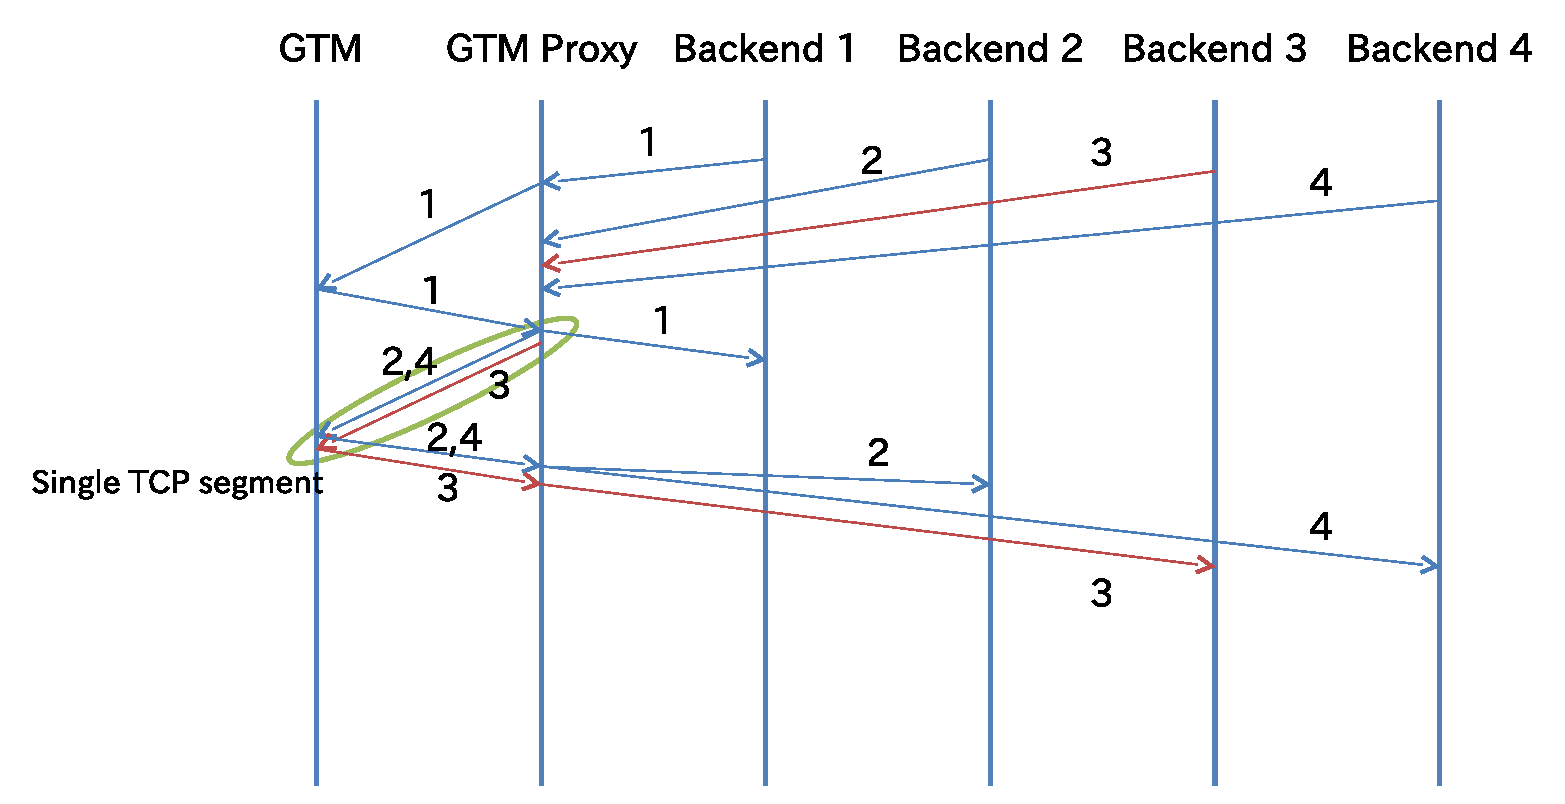
\includegraphics[width=0.9\hsize]{txn_gtmpxy.eps}
		  \caption{\label{fig:txngtmpxy}Example of GTM Proxy}
	  \end{center}
  \end{figure}
  
  These characteristics are brought from the internal structure of the GTM proxy.
  
  The GTM proxy is implemented with the worker thread model, and single thread handles multiple
  connections from the backends and single connection to GTM.
  After the main server loop \file{src/gtm/proxy/proxy_main.c:ServerLoop()} accepts a connection
  from a backend, the connection is dispatched to worker process in
  \file{proxy_main.c:GTMProxyAddConnection()}.
  The example used one worker thread.
  
  \file{proxy_main.c:GTMProxy_ThreadMain()} is the main loop of worker threads.
  This loop has two phases.

  1st phase reads data from all backend connections, and call \file{ProcessCommand()} to dispatch
  received message to \texttt{Process\textit{XXXXXXXX}Command()}.
  If the message is packable, \texttt{Processi\textit{XXXXXXXX}Command()} calls
  \file{GTMProxy_CommandPending()} to store the information.
  If the message is not packaged, {\tt } calls \file{GTMProxy_ProxyCommand()} to propagate the
  message immediately to GTM.
  Please note that the response is not received here.
  When all connections has no pending data, received messages are packed into single message,
  which is send it to the GTM.
  
  2nd phase reads data from the GTM connection and call \file{ProcessResponse()} to distribute
  received response to the backends.
  2nd phase is repeated until all response correspond to the message received in 1st phase.
  
  Because GTM proxy groups more than one message from coordinator/datanode backend into single
  packed message, it needs dedicated error handling.
  GTM protocol was extended to handle this.
  Without GTM proxy, GTM had direct connection to the backend.
  So the GTM automatically aborted transaction to cleanup transactions implicitly aborted when
  the connection is disconnected.
  With the GTM proxy, the GTM proxy holds connection even if one of the backend's connection
  handled by a thread disconnected.
  To avoid the transaction is left, the some packed message includes connection ID that identify
  the connection received the message.
  And the GTM proxy sends \file{MSG_BACKEND_DISCONNECT} to notify a disconnection of a backend.
  Please note that \file{MSG_BACKEND_DISCONNECT} message's body doesn't have connection ID.
  The message notifies the connection ID using \file{ProxyHdr} which is inserted to every message's
  body by the GTM proxy.

